\PassOptionsToPackage{xcolor}{usenames,dvipsnames,svgnames,table}
\documentclass[10pt]{report}
\usepackage[T1]{fontenc}
\usepackage{lmodern}
\usepackage{pdfcolmk}
\usepackage{multirow}
\usepackage{graphicx}
\usepackage{pifont}
\usepackage{amsmath,amsfonts,amsthm,amssymb}
\usepackage{setspace}
\usepackage{Tabbing}
\usepackage{etoolbox}
\usepackage{fancyhdr}
\usepackage{lastpage}
\usepackage{listings}
\usepackage{extramarks}
\usepackage{enumerate}
\usepackage{soul,color}
\usepackage{graphicx,float,wrapfig}
\usepackage{amsmath,amssymb,rotating}
\usepackage{epsfig}
\usepackage{color}
\usepackage{hyperref}
\usepackage{animate}
\usepackage{array}
\usepackage{graphics, color}
\usepackage{graphicx}
\usepackage{epsfig}
\usepackage{setspace}
\usepackage{verbatim}
\usepackage[margin=1.0in]{geometry}
\usepackage{tikz}
\usepackage{mdframed}
\usepackage{clrscode3e}
\usepackage{formalHW}
\usepackage[none,DMC]{formatHW}
\usepackage{fancyquote}
\usepackage{fancyenvironments}
\usepackage{mymathmacros}
\usepackage{algorithm}
\usepackage[noend]{algpseudocode}
\usepackage{pgfplots}

%set up fancy page header
\pagestyle{fancy}
   \chead{DMC@ISU:\ Too many features}  
   \rhead{\firstxmark}
   \lfoot{\lastxmark}
   \cfoot{}
   \rfoot{Page\ \thepage\ of\ \pageref{LastPage}}
   \renewcommand\headrulewidth{0.4pt}
   \renewcommand\footrulewidth{0.4pt}

% pandoc syntax highlighting
\usepackage{color}
\usepackage{fancyvrb}
\newcommand{\VerbBar}{|}
\newcommand{\VERB}{\Verb[commandchars=\\\{\}]}
\DefineVerbatimEnvironment{Highlighting}{Verbatim}{commandchars=\\\{\}}
% Add ',fontsize=\small' for more characters per line
\newenvironment{Shaded}{}{}
\newcommand{\KeywordTok}[1]{\textcolor[rgb]{0.00,0.44,0.13}{\textbf{{#1}}}}
\newcommand{\DataTypeTok}[1]{\textcolor[rgb]{0.56,0.13,0.00}{{#1}}}
\newcommand{\DecValTok}[1]{\textcolor[rgb]{0.25,0.63,0.44}{{#1}}}
\newcommand{\BaseNTok}[1]{\textcolor[rgb]{0.25,0.63,0.44}{{#1}}}
\newcommand{\FloatTok}[1]{\textcolor[rgb]{0.25,0.63,0.44}{{#1}}}
\newcommand{\CharTok}[1]{\textcolor[rgb]{0.25,0.44,0.63}{{#1}}}
\newcommand{\StringTok}[1]{\textcolor[rgb]{0.25,0.44,0.63}{{#1}}}
\newcommand{\CommentTok}[1]{\textcolor[rgb]{0.38,0.63,0.69}{\textit{{#1}}}}
\newcommand{\OtherTok}[1]{\textcolor[rgb]{0.00,0.44,0.13}{{#1}}}
\newcommand{\AlertTok}[1]{\textcolor[rgb]{1.00,0.00,0.00}{\textbf{{#1}}}}
\newcommand{\FunctionTok}[1]{\textcolor[rgb]{0.02,0.16,0.49}{{#1}}}
\newcommand{\RegionMarkerTok}[1]{{#1}}
\newcommand{\ErrorTok}[1]{\textcolor[rgb]{1.00,0.00,0.00}{\textbf{{#1}}}}
\newcommand{\NormalTok}[1]{{#1}}

% header includes

\begin{document}

\thispagestyle{empty}%
\begin{center}%
    \renewcommand{\arraystretch}{1.5}%
    \begin{tabular}{c}%
       \Large{DMC@ISU: The 2015 Iowa State University Data Mining Cup Team}\\
       Curation and Cross Validation to Reduce Features\\
       Spring 2015, A Team as Strong as Steel \\
    \end{tabular}
\end{center}

\begin{center}
 \renewcommand{\arraystretch}{1.5}
 \begin{tabular*}{0.65\textwidth}{r@{:\hspace{.3cm}}l}
    \hline
    
    
    Last Day&  May 19, 2015\\
    \hline
 \end{tabular*}
\end{center}

I am using the following packages:

\begin{Shaded}
\begin{Highlighting}[]
   \KeywordTok{library}\NormalTok{(magrittr)}
   \KeywordTok{library}\NormalTok{(dplyr)}
   \KeywordTok{library}\NormalTok{(reshape2)}
   \KeywordTok{library}\NormalTok{(tidyr)}
   \KeywordTok{library}\NormalTok{(lubridate)}
   \KeywordTok{library}\NormalTok{(ggplot2)}
   \KeywordTok{library}\NormalTok{(directlabels)}
   \KeywordTok{library}\NormalTok{(rCharts)}
   \KeywordTok{library}\NormalTok{(xtable)}
   \KeywordTok{library}\NormalTok{(foreach)}
   \KeywordTok{library}\NormalTok{(gtools)}
   \KeywordTok{library}\NormalTok{(knitr)}
   \KeywordTok{library}\NormalTok{(utils)}
   \KeywordTok{source}\NormalTok{(}\StringTok{"~/dmc2015/ian/R/renm.R"}\NormalTok{)}
\end{Highlighting}
\end{Shaded}

My working directory is set to \verb!~/dmc2015/ian/!.

\section{Curating and Cross
Validating}\label{curating-and-cross-validating}

The reason features should be removed from an ``large data'' approach to
a problem is if they are dominated by better features.

However, when you have as many features as we do at the moment it can be
difficult to

I am starting with \textbf{set 1}

\section{Load feature matrix}\label{load-feature-matrix}

\begin{Shaded}
\begin{Highlighting}[]
\NormalTok{## long}
\NormalTok{f1 =}\StringTok{ }\KeywordTok{readRDS}\NormalTok{(}\StringTok{"../data/featureMatrix/featMat_based-on-HTVset1_LONG_ver0.3.rds"}\NormalTok{)}

\NormalTok{## wide}
\NormalTok{d1 =}\StringTok{ }\KeywordTok{readRDS}\NormalTok{(}\StringTok{"../data/featureMatrix/featMat_based-on-HTVset1_WIDE_ver0.3.rds"}\NormalTok{)}
\end{Highlighting}
\end{Shaded}

\section{Check the data}\label{check-the-data}

\begin{Shaded}
\begin{Highlighting}[]
\NormalTok{## isolate the X and y for set 1}
\NormalTok{Xn =}\StringTok{ }\NormalTok{f1$train$X}
\NormalTok{yn =}\StringTok{ }\NormalTok{f1$train$y}

\NormalTok{## remove the naive columns}
\NormalTok{Xn =}\StringTok{ }\NormalTok{Xn[, !}\KeywordTok{grepl}\NormalTok{(}\StringTok{"naive"}\NormalTok{, }\KeywordTok{names}\NormalTok{(Xn))]}

\NormalTok{## keep the validation sets}
\NormalTok{Xv =}\StringTok{ }\NormalTok{f1$validation$X}
\NormalTok{yv =}\StringTok{ }\NormalTok{f1$validation$y}
\end{Highlighting}
\end{Shaded}

And this is our loss function:

\begin{Shaded}
\begin{Highlighting}[]
\NormalTok{lossFunMethod =}\StringTok{ }\NormalTok{function(yval, Xval, method) \{}
    \NormalTok{hatmat =}\StringTok{ }\KeywordTok{as.matrix}\NormalTok{(}\KeywordTok{matrix}\NormalTok{(}\KeywordTok{predict}\NormalTok{(method, }\DataTypeTok{newdata =} \NormalTok{Xval, }\DataTypeTok{type =} \StringTok{"response"}\NormalTok{), }
        \DataTypeTok{ncol =} \DecValTok{3}\NormalTok{, }\DataTypeTok{byrow =} \OtherTok{TRUE}\NormalTok{))}
    \NormalTok{ymat =}\StringTok{ }\KeywordTok{matrix}\NormalTok{(yval, }\DataTypeTok{ncol =} \DecValTok{3}\NormalTok{, }\DataTypeTok{byrow =} \OtherTok{TRUE}\NormalTok{)}
    
    \NormalTok{error =}\StringTok{ }\KeywordTok{colSums}\NormalTok{((ymat -}\StringTok{ }\NormalTok{hatmat)^}\DecValTok{2}\NormalTok{)}
    \NormalTok{wt =}\StringTok{ }\KeywordTok{colMeans}\NormalTok{(ymat)^}\DecValTok{2}
    
    \KeywordTok{cat}\NormalTok{(}\StringTok{"The coupon error is:  "}\NormalTok{, }\KeywordTok{sum}\NormalTok{(error/wt), }\StringTok{"}\CharTok{\textbackslash{}n}\StringTok{"}\NormalTok{)}
    \KeywordTok{cat}\NormalTok{(}\StringTok{"By column error:      "}\NormalTok{, error, }\StringTok{"}\CharTok{\textbackslash{}n}\StringTok{"}\NormalTok{)}
    \KeywordTok{cat}\NormalTok{(}\StringTok{"By column weight:     "}\NormalTok{, wt, }\StringTok{"}\CharTok{\textbackslash{}n\textbackslash{}n}\StringTok{"}\NormalTok{)}
    \KeywordTok{return}\NormalTok{(}\KeywordTok{sum}\NormalTok{(error/wt))}
\NormalTok{\}}
\end{Highlighting}
\end{Shaded}

The following functions will help me in this process:

\begin{Shaded}
\begin{Highlighting}[]
\NormalTok{## I will use cross validation to estimate an error instead of checking the}
\NormalTok{## validation set}
\NormalTok{RFxVal =}\StringTok{ }\NormalTok{function(CVk, Xrf, yrf, }\DataTypeTok{mtry =} \DecValTok{8}\NormalTok{, }\DataTypeTok{ntree =} \DecValTok{1000}\NormalTok{, }\DataTypeTok{maxnodes =} \DecValTok{50}\NormalTok{) \{}
    \NormalTok{row.order =}\StringTok{ }\KeywordTok{sample}\NormalTok{(}\DecValTok{1}\NormalTok{:}\KeywordTok{nrow}\NormalTok{(Xrf))}
    \NormalTok{CV.bounds =}\StringTok{ }\KeywordTok{round}\NormalTok{(}\KeywordTok{seq.int}\NormalTok{(}\DecValTok{1}\NormalTok{, }\KeywordTok{nrow}\NormalTok{(Xrf), }\DataTypeTok{length =} \NormalTok{(CVk +}\StringTok{ }\DecValTok{1}\NormalTok{)))}
    \NormalTok{OOBset =}\StringTok{ }\KeywordTok{lapply}\NormalTok{(}\DecValTok{1}\NormalTok{:CVk, function(i) row.order[CV.bounds[}\DecValTok{1}\NormalTok{]:(CV.bounds[}\DecValTok{2}\NormalTok{] -}\StringTok{ }
\StringTok{        }\DecValTok{1}\NormalTok{)])}
    
    \CommentTok{# Fit a random forest for couponUsed}
    \NormalTok{cvRF =}\StringTok{ }\NormalTok{function(rows) }\KeywordTok{randomForest}\NormalTok{(Xrf[-rows, ], }\DataTypeTok{y =} \NormalTok{yrf[-rows], }\DataTypeTok{ntree =} \NormalTok{ntree, }
        \DataTypeTok{mtry =} \NormalTok{mtry, }\DataTypeTok{replace =} \OtherTok{TRUE}\NormalTok{, }\DataTypeTok{maxnodes =} \NormalTok{maxnodes)}
    
    \KeywordTok{message}\NormalTok{(}\StringTok{"Fitting randomForest"}\NormalTok{)}
    \NormalTok{rf_cvs =}\StringTok{ }\KeywordTok{lapply}\NormalTok{(}\DecValTok{1}\NormalTok{:CVk, function(i) }\KeywordTok{cvRF}\NormalTok{(OOBset[[i]]))}
    
    \KeywordTok{message}\NormalTok{(}\StringTok{"Calculating Loss"}\NormalTok{)}
    \NormalTok{lossFunction =}\StringTok{ }\KeywordTok{lapply}\NormalTok{(}\DecValTok{1}\NormalTok{:CVk, function(i) }\KeywordTok{lossFunMethod}\NormalTok{(yrf[OOBset[[i]]], }
        \NormalTok{Xrf[OOBset[[i]], ], rf_cvs[[i]]))}
    
    \KeywordTok{print}\NormalTok{(lossFunction)}
    \KeywordTok{return}\NormalTok{(rf_cvs)}
\NormalTok{\}}

\NormalTok{## CV to get the mean importance}
\NormalTok{RFxVal_imp =}\StringTok{ }\NormalTok{function(RFs) \{}
    \NormalTok{RFimp =}\StringTok{ }\KeywordTok{data.frame}\NormalTok{(}\DataTypeTok{feature =} \KeywordTok{rownames}\NormalTok{(RFs[[}\DecValTok{1}\NormalTok{]]$importance), }\DataTypeTok{IncNodePurity1 =} \NormalTok{RFs[[}\DecValTok{1}\NormalTok{]]$importance)}
    \KeywordTok{rownames}\NormalTok{(RFimp) =}\StringTok{ }\OtherTok{NULL}
    \KeywordTok{names}\NormalTok{(RFimp) =}\StringTok{ }\KeywordTok{c}\NormalTok{(}\StringTok{"feature"}\NormalTok{, }\StringTok{"IncNodePurity1"}\NormalTok{)}
    \NormalTok{for (i in }\DecValTok{2}\NormalTok{:}\KeywordTok{length}\NormalTok{(RFs)) \{}
        \NormalTok{RFimp.i =}\StringTok{ }\KeywordTok{data.frame}\NormalTok{(}\DataTypeTok{feature =} \KeywordTok{rownames}\NormalTok{(RFs[[i]]$importance), }\DataTypeTok{IncNodePurity1 =} \NormalTok{RFs[[i]]$importance)}
        \KeywordTok{names}\NormalTok{(RFimp.i) =}\StringTok{ }\KeywordTok{c}\NormalTok{(}\StringTok{"feature"}\NormalTok{, }\KeywordTok{paste0}\NormalTok{(}\StringTok{"IncNodePurity"}\NormalTok{, i))}
        \KeywordTok{rownames}\NormalTok{(RFimp.i) =}\StringTok{ }\OtherTok{NULL}
        \NormalTok{RFimp =}\StringTok{ }\NormalTok{RFimp %>%}\StringTok{ }\KeywordTok{left_join}\NormalTok{(RFimp.i, }\DataTypeTok{by =} \StringTok{"feature"}\NormalTok{)}
    \NormalTok{\}}
    \NormalTok{RFimplong =}\StringTok{ }\NormalTok{RFimp %>%}\StringTok{ }\KeywordTok{gather}\NormalTok{(colname, IncNodePurity, -feature) %>%}\StringTok{ }\KeywordTok{mutate}\NormalTok{(}\DataTypeTok{CViteration =} \KeywordTok{as.numeric}\NormalTok{(}\KeywordTok{gsub}\NormalTok{(}\StringTok{"IncNodePurity"}\NormalTok{, }
        \StringTok{""}\NormalTok{, colname))) %>%}\StringTok{ }\KeywordTok{select}\NormalTok{(feature, CViteration, IncNodePurity) %>%}\StringTok{ }\KeywordTok{arrange}\NormalTok{(feature, }
        \NormalTok{CViteration)}
    
    \NormalTok{RFimplongMeans =}\StringTok{ }\NormalTok{RFimplong %>%}\StringTok{ }\KeywordTok{group_by}\NormalTok{(feature) %>%}\StringTok{ }\KeywordTok{summarize}\NormalTok{(}\DataTypeTok{meanIncNodePurity =} \KeywordTok{mean}\NormalTok{(IncNodePurity))}
    
    \NormalTok{CVimpplotfunc =}\StringTok{ }\NormalTok{function(dsn) \{}
        \NormalTok{CVplot =}\StringTok{ }\KeywordTok{ggplot}\NormalTok{(}\DataTypeTok{data =} \NormalTok{dsn, }\KeywordTok{aes}\NormalTok{(}\DataTypeTok{x =} \NormalTok{CViteration, }\DataTypeTok{y =} \NormalTok{IncNodePurity, }
            \DataTypeTok{group =} \NormalTok{feature, }\DataTypeTok{color =} \NormalTok{feature)) +}\StringTok{ }\KeywordTok{geom_line}\NormalTok{() +}\StringTok{ }\KeywordTok{theme}\NormalTok{(}\DataTypeTok{legend.position =} \StringTok{"none"}\NormalTok{) +}\StringTok{ }
\StringTok{            }\KeywordTok{geom_text}\NormalTok{(}\DataTypeTok{data =} \NormalTok{RFimplong[RFimplong$CViteration ==}\StringTok{ }\DecValTok{1}\NormalTok{, ], }\KeywordTok{aes}\NormalTok{(}\DataTypeTok{label =} \NormalTok{feature), }
                \DataTypeTok{hjust =} \DecValTok{1}\NormalTok{, }\DataTypeTok{size =} \FloatTok{0.1}\NormalTok{)}
        \NormalTok{CVplot =}\StringTok{ }\KeywordTok{direct.label}\NormalTok{(CVplot +}\StringTok{ }\KeywordTok{xlim}\NormalTok{(}\DecValTok{0}\NormalTok{, }\KeywordTok{length}\NormalTok{(RFs) +}\StringTok{ }\DecValTok{10}\NormalTok{), }\StringTok{"last.qp"}\NormalTok{)}
        \KeywordTok{return}\NormalTok{(CVplot)}
    \NormalTok{\}}
    
    \NormalTok{RFimp =}\StringTok{ }\KeywordTok{list}\NormalTok{(}\DataTypeTok{importance =} \NormalTok{RFimp, }\DataTypeTok{iterations =} \NormalTok{RFimplong, }\DataTypeTok{mean =} \NormalTok{RFimplongMeans, }
        \DataTypeTok{plot =} \KeywordTok{CVimpplotfunc}\NormalTok{(RFimplong), }\DataTypeTok{makeplot =} \NormalTok{CVimpplotfunc)}
    
    \KeywordTok{return}\NormalTok{(RFimp)}
\NormalTok{\}}
\end{Highlighting}
\end{Shaded}

\section{I am going to start with a simple random
forest}\label{i-am-going-to-start-with-a-simple-random-forest}

\begin{Shaded}
\begin{Highlighting}[]
\NormalTok{set.seed =}\StringTok{ }\DecValTok{1999}
\NormalTok{## lets try a small random forest}
\KeywordTok{library}\NormalTok{(randomForest)}
\end{Highlighting}
\end{Shaded}

\begin{verbatim}
## randomForest 4.6-10
## Type rfNews() to see new features/changes/bug fixes.
## 
## Attaching package: 'randomForest'
## 
## The following object is masked from 'package:dplyr':
## 
##     combine
\end{verbatim}

\begin{Shaded}
\begin{Highlighting}[]
\NormalTok{## get the similarity columns}
\NormalTok{sim_columns =}\StringTok{ }\KeywordTok{c}\NormalTok{(}\DecValTok{3}\NormalTok{, }\KeywordTok{grep}\NormalTok{(}\StringTok{"sim_"}\NormalTok{, }\KeywordTok{names}\NormalTok{(Xn)))}

\NormalTok{## get single way llrs:}
\NormalTok{llr1_columns =}\StringTok{ }\KeywordTok{which}\NormalTok{(}\KeywordTok{grepl}\NormalTok{(}\StringTok{"llr"}\NormalTok{, }\KeywordTok{names}\NormalTok{(Xn)) &}\StringTok{ }\NormalTok{!}\KeywordTok{grepl}\NormalTok{(}\StringTok{"X"}\NormalTok{, }\KeywordTok{names}\NormalTok{(Xn)))}

\CommentTok{# The predictor and response columns}
\NormalTok{Xrf =}\StringTok{ }\NormalTok{Xn[, }\KeywordTok{c}\NormalTok{(sim_columns, llr1_columns)]}

\NormalTok{## I will use cross validation to estimate an error instead of checking the}
\NormalTok{## validation set}
\NormalTok{set.seed =}\StringTok{ }\DecValTok{1999}
\NormalTok{CVrf =}\StringTok{ }\KeywordTok{RFxVal}\NormalTok{(}\DecValTok{5}\NormalTok{, Xrf, yn[, }\StringTok{"couponUsed"}\NormalTok{], }\DataTypeTok{mtry =} \DecValTok{8}\NormalTok{, }\DataTypeTok{ntree =} \DecValTok{1000}\NormalTok{, }\DataTypeTok{maxnodes =} \DecValTok{50}\NormalTok{)}
\end{Highlighting}
\end{Shaded}

\begin{verbatim}
## Fitting randomForest
\end{verbatim}

\begin{verbatim}
## Warning in randomForest.default(Xrf[-rows, ], y = yrf[-rows], ntree =
## ntree, : The response has five or fewer unique values.  Are you sure you
## want to do regression?
\end{verbatim}

\begin{verbatim}
## Warning in randomForest.default(Xrf[-rows, ], y = yrf[-rows], ntree =
## ntree, : The response has five or fewer unique values.  Are you sure you
## want to do regression?
\end{verbatim}

\begin{verbatim}
## Warning in randomForest.default(Xrf[-rows, ], y = yrf[-rows], ntree =
## ntree, : The response has five or fewer unique values.  Are you sure you
## want to do regression?
\end{verbatim}

\begin{verbatim}
## Warning in randomForest.default(Xrf[-rows, ], y = yrf[-rows], ntree =
## ntree, : The response has five or fewer unique values.  Are you sure you
## want to do regression?
\end{verbatim}

\begin{verbatim}
## Warning in randomForest.default(Xrf[-rows, ], y = yrf[-rows], ntree =
## ntree, : The response has five or fewer unique values.  Are you sure you
## want to do regression?
\end{verbatim}

\begin{verbatim}
## Calculating Loss
\end{verbatim}

\begin{verbatim}
## The coupon error is:   5471.761 
## By column error:       78.29988 81.46362 86.24724 
## By column weight:      0.04180429 0.04180429 0.05226918 
## 
## The coupon error is:   5475.783 
## By column error:       78.43724 81.5225 86.21214 
## By column weight:      0.04180429 0.04180429 0.05226918 
## 
## The coupon error is:   5472.216 
## By column error:       78.36817 81.3622 86.31244 
## By column weight:      0.04180429 0.04180429 0.05226918 
## 
## The coupon error is:   5477.79 
## By column error:       78.34235 81.58994 86.35134 
## By column weight:      0.04180429 0.04180429 0.05226918 
## 
## The coupon error is:   5474.873 
## By column error:       78.21605 81.57335 86.37757 
## By column weight:      0.04180429 0.04180429 0.05226918 
## 
## [[1]]
## [1] 5471.761
## 
## [[2]]
## [1] 5475.783
## 
## [[3]]
## [1] 5472.216
## 
## [[4]]
## [1] 5477.79
## 
## [[5]]
## [1] 5474.873
\end{verbatim}

\begin{Shaded}
\begin{Highlighting}[]
\NormalTok{CVimp =}\StringTok{ }\KeywordTok{RFxVal_imp}\NormalTok{(CVrf)}
\end{Highlighting}
\end{Shaded}

\begin{verbatim}
## Loading required package: proto
\end{verbatim}

\begin{Shaded}
\begin{Highlighting}[]
\NormalTok{CVimp$plot}

\NormalTok{CVimp$}\KeywordTok{makeplot}\NormalTok{(CVimp$iteration[}\KeywordTok{which}\NormalTok{(CVimp$iteration$IncNodePurity >}\StringTok{ }\DecValTok{1}\NormalTok{), ])}

\CommentTok{# fit full data}
\NormalTok{rf1 =}\StringTok{ }\KeywordTok{randomForest}\NormalTok{(Xrf, }\DataTypeTok{y =} \NormalTok{yn$couponUsed, }\DataTypeTok{ntree =} \DecValTok{1000}\NormalTok{, }\DataTypeTok{mtry =} \DecValTok{8}\NormalTok{, }\DataTypeTok{replace =} \OtherTok{TRUE}\NormalTok{, }
    \DataTypeTok{maxnodes =} \DecValTok{50}\NormalTok{)}
\end{Highlighting}
\end{Shaded}

\begin{verbatim}
## Warning in randomForest.default(Xrf, y = yn$couponUsed, ntree = 1000, mtry
## = 8, : The response has five or fewer unique values.  Are you sure you
## want to do regression?
\end{verbatim}

\begin{Shaded}
\begin{Highlighting}[]
\CommentTok{# get the output}
\KeywordTok{lossFunMethod}\NormalTok{(yv$couponUsed, Xv[, }\KeywordTok{which}\NormalTok{(}\KeywordTok{names}\NormalTok{(Xv) %in%}\StringTok{ }\KeywordTok{names}\NormalTok{(Xrf))], rf1)}
\end{Highlighting}
\end{Shaded}

\begin{verbatim}
## The coupon error is:   16557.93 
## By column error:       221.7057 174.9989 165.6331 
## By column weight:      0.05660508 0.02898854 0.02507926
\end{verbatim}

\begin{verbatim}
## [1] 16557.93
\end{verbatim}

\begin{center}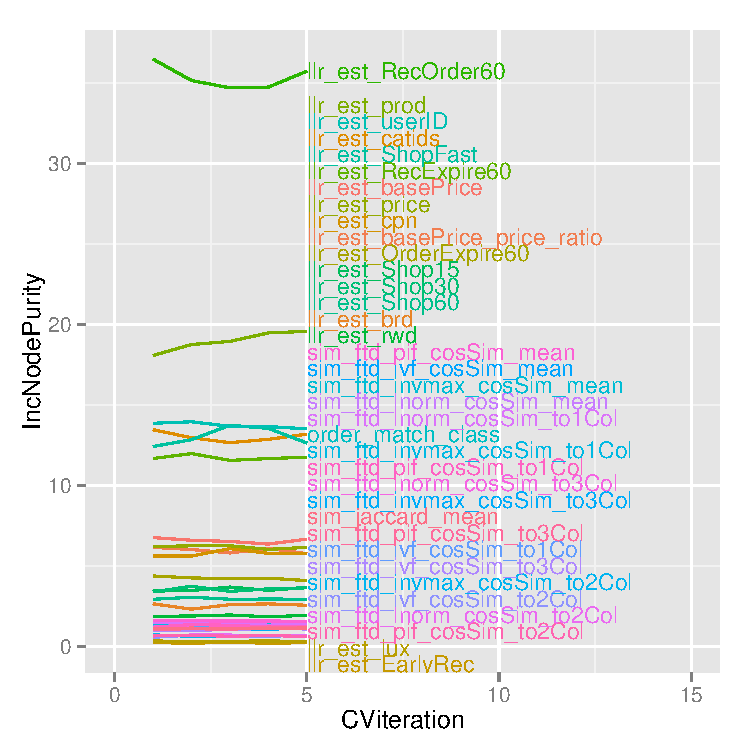
\includegraphics{/Users/user/dmc2015/ian/graphics/fig_rf-1} 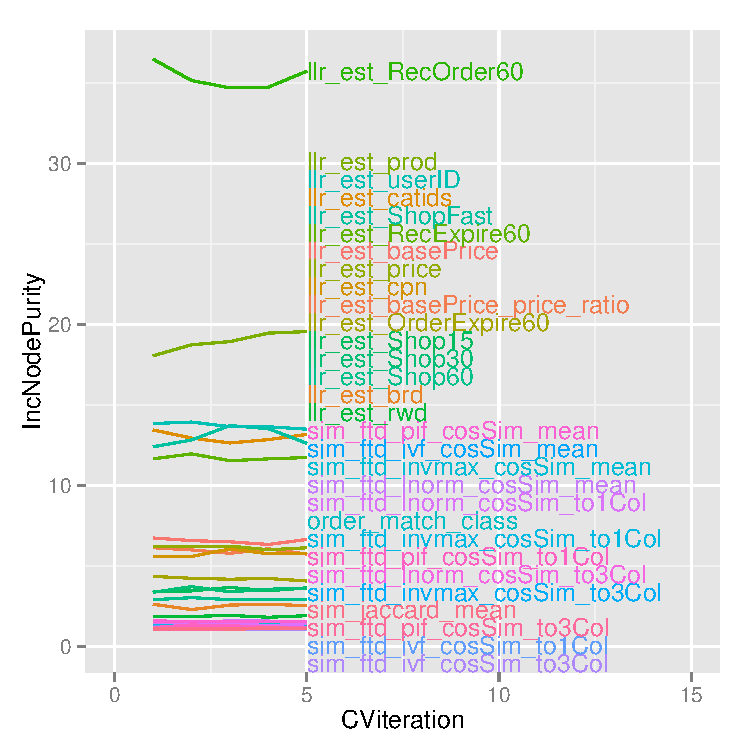
\includegraphics{/Users/user/dmc2015/ian/graphics/fig_rf-2} \end{center}

\end{document}
